\documentclass[12pt]{article}

\usepackage[margin=1.0in]{geometry}
\usepackage{graphicx}
\usepackage{tabto}
\graphicspath{ {./} }

\begin{document}

\title{CS4348 : Operating Systems Concepts\\Homework Assignment 3}
\author{Matthew McMillian\\mgm160130@utdallas.edu}
\maketitle

\begin{enumerate}

	\item How does interrupt disabling provide mutual exclusion? \\ \\
	Assuming that we are not threading, interrupt disabling proves mutual exclusion since there is only one way line of execution for the program to perform. This means that control over a resource can never be 'taken away'. Take for example if we are currently in a write operation to a file. If an interrupt were to happen, we would lose our access to that resource and data could get corrupted. By disabling interrupts, we can enforce the idea that if we are in critical sections that we will only have one way to exit the critical section; by completing the task.
	
	\item In the Compare$\&$Swap instruction, why must the instruction execute atomically? \\ \\
	Since we are using using our dynamic variable $x$ inside the compare$\_$and$\_$swap method and setting it afterwords, there is a chance that we set $x$ before the comparison has even been made. Therefore in order to preserve the integrity of our data, we must make each method atomic so that our data doesn't get interleaved / interchanged by accident.
	
	\item Coordinate the actions of the two threads below by inserting wait/signal commands on semaphores so that the Give$\_$order() happens first, then the Take$\_$order(), then the Serve$\_$meal(), then the Eat$\_$meal().  You can assume one thread each.
    \begin{center}
    binary$\_$semaphore s.order = 1 \\
    binary$\_$sempahore s.order.delay = 0 \\ 
    binary$\_$semaphore s.meal = 0 \\
     Customer  \tabto{4cm}         Waiter\\
	 wait(s.order)	\tabto{4cm}		  wait(s.order.delay) \\
     Give$\_$order() \tabto{4cm}      Take$\_$order() \\
	 signal(s.order.delay) \tabto{4cm} Serve$\_$meal()\\
	 wait(s.meal)	\tabto{4cm}		  signal(s.meal)\\
     Eat$\_$meal()   \tabto{4cm}      Serve$\_$meal()\\
	 signal(s.meal) \tabto{4cm}	      signal(s.order) \\
    \end{center}
    
   \item Why is the mutual exclusion condition necessary for deadlock to occur? \\ \\
   The whole reason behind a deadlock is that other processes are waiting on each other to use a resource. If there is no mutual exclusion, then there is no need to wait on other processes, and as such there wouldn't be any deadlock. Consider the case used in the first problem where we are waiting on a file to read/write from. If there is no mutual exclusion, then another process could just write to the file at the same time as the original process (though this is unsafe, a deadlock wouldn't occur). 
   
   \item Suppose there are three processes, P1, P2, and P3, and three files, FileA, FileB, and FileC. P1 has FileA and wants FileC.  P2 has FileB and wants FileA.  P3 has FileC and wants FileB.  \\
   a) Draw a resource allocation graph for this situation.
   \begin{center}
   	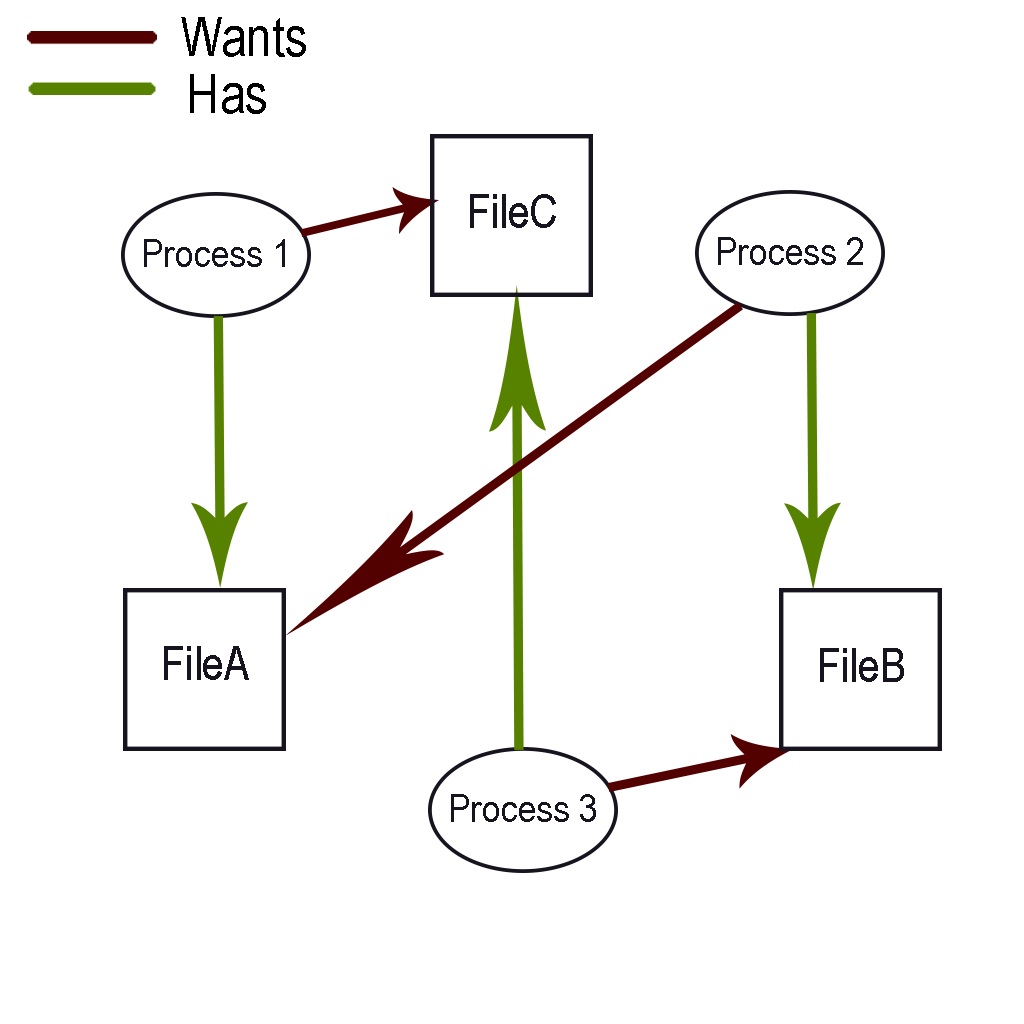
\includegraphics[scale=0.35]{dependency}
   \end{center}
   b) Does the graph represent a deadlock?  Why or why not? Explain.\\ \\
   Yes, this resource allocation graph represents a deadlock. Each process (independently) has every resource available, and each process wants an resource currently being held by another process, and as such was have resulting in a deadlock.
   
   \item Is the following setup safe or unsafe according to the Banker's algorithm? Show your work and explain your result. \\ \\
	The following setup is unsafe according to the Banker's algorithm. Since we currently have no available R1 resources, and because we cannot free up any other process with the resources we have available, there will be a potential deadlock (unsafe) operation that could occur.       
      
\end{enumerate}
\end{document}
